\section{Wrapping up the deal}

Before we draft the legal documents, we need to agree on the most important
principles of the deal:
\begin{itemize}
    \item The amount invested, and how it will be made available (in one single
        payment, or in tranches dependent on milestones)
    \item The value of the company (with a distinction between pre- and post money
        valuation)
    \item The cap table, who owns what percentage of the company
    \item The Governance principles
\end{itemize}

\subsection{The amount invested}

In the example of Company $X$, we decided to invest $2$M Euro's. This was
our base case scenario. The investment amount turned out to be too small
and follow up rounds were needed. Investors may have an incentive to start
with a low initial investment, if things go well they will have a higher
ROI, if things go bad, they can invest the additional amount at a lower
company valuation. As a founder/entrepreneur, it is important to negotiate
for a strong cash buffer. If the cash burn is higher than expected, you may
need to find new capital in a situation under stress. At that time your
company valuation will be lower and you will dilute (start losing ownership
of the company).

\subsection{Value of the Company}

\begin{figure}[H]
    \centering
    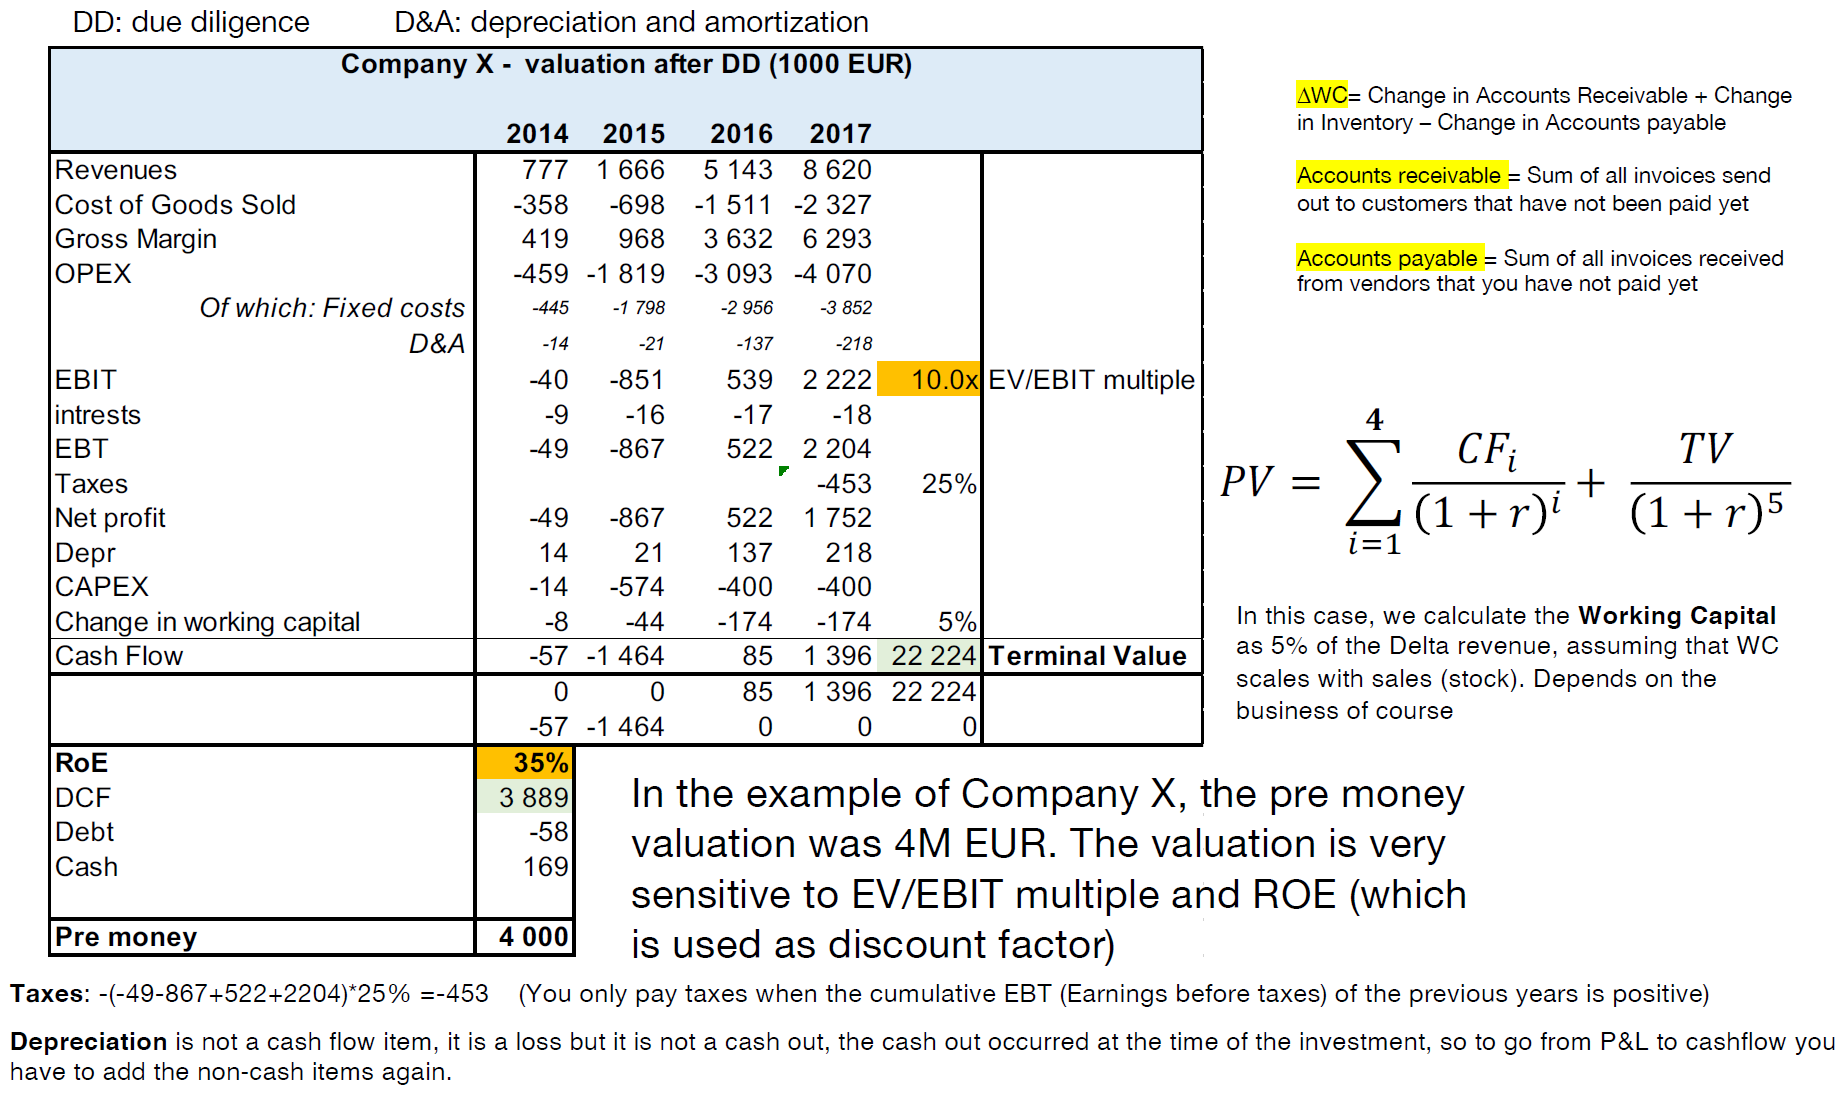
\includegraphics[width=0.9\textwidth]{Pictures/value_of_the_company.png}
    \caption{Value of the Company}
\end{figure}

\begin{figure}[H]
    \centering
    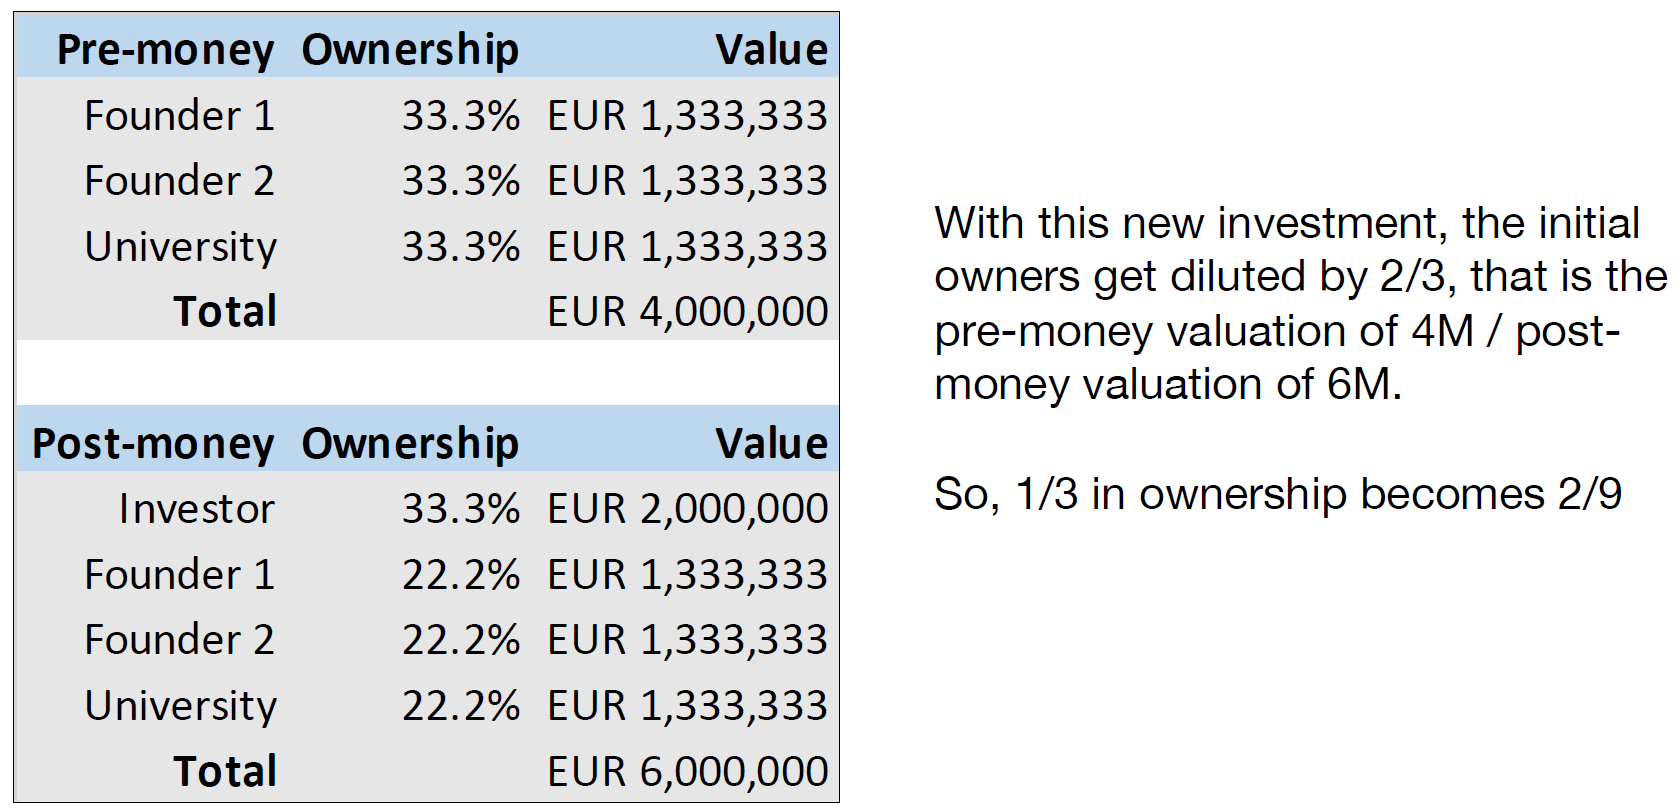
\includegraphics[width=0.6\textwidth]{Pictures/pre_and_post_money.png}
    \caption{Pre- and Post money}
\end{figure}

\subsection{Cap Table}

Capitalization Table: Specifying ownerships, equity value, etc.

\subsubsection{Governance principles}

\begin{enumerate}[]
    \item \underline{What?}: To outline the responsibility, the composition and the
        authority (the decisions making process) of the Management Team (MT), the
        Supervisory Board (SVB) and the General Meeting of Shareholders (GMS) of
        the company.
    \item \underline{Why?}: To allow for an efficient management of the company
        based on objective criteria and processes independently of existing persons
        and historical relationships.
    \item \underline{How?}: By writing or changing the article of association and/or
        the shareholder agreement, where needed.
\end{enumerate}

\subsubsection{Corporate Bodies}

Consists of three parts: General Meeting of Shareholders, Supervisory Board,
Management Team.

\paragraph{Management Team} Day-to-Day affairs

\begin{itemize}
    \item Directs the company's day-to-day affairs
    \item Has the authority to decide in line with the annual budget and business
        plan that has been approved by the board.
    \item In case of significant deviation from the budget and the business plan,
        the decision is escalated to the board.
    \item Often a matrix is drafted showing clearly the decision authority
        of each or multiple MT members ordered according to subject, amount,
        signing authority \dots
\end{itemize}

\paragraph{Supervisory Board} Supervision

\begin{itemize}
    \item Composed of representatives of the shareholders + independent board
        members (non-executive) + senior management (executive)
    \item Composition and voting rights are clearly defined in the shareholders
        agreement.
    \item Must supervise and advise the management and oversee the general affairs
        within the company.
    \item Should be guided by the interests of the company.
\end{itemize}

\paragraph{Supervisory Board, Typical decision authority of the board}

\begin{itemize}
    \item Hire/fire of senior management
    \item Adoption and/or amendment of yearly business plan and budget
    \item Investment, loans, contracts \dots exceeding a threshold
    \item Option plan for employees
    \item Targets and variable remuneration of senior management
\end{itemize}

\paragraph{General meeting of Shareholders} Value creation

\begin{itemize}
    \item Composed of the shareholders (owners) of the company
    \item May give priority to their own interests with due regard for the
        principles of reasonableness and fairness
    \item Meets at least once per year to approve the annual accounts,
        discharge the board and follow up and/or adapt the Value Creation
        Plan (long term business plan)
    \item Appoints the members of the Supervisory Board and sometimes also
        members of the management team (like the CEO)
    \item Decides by majority unless explicity stated differently in the
        shareholder agreement.
\end{itemize}

\paragraph{General meeting of Shareholders, Typical decision authority
of shareholders:}

\begin{itemize}
    \item issue of new shares
    \item hire/fire new CEO
    \item distribution of dividends
    \item Reorganisation of the business
    \item Application for bankruptcy
    \item Debt restructuring
    \item Acquisition of another company
    \item Sale to - or merger with another company
    \item \dots
\end{itemize}

\subsubsection{Legal Documents}

Once the amount invested, the value of the company, the cap table, and the
governance principles are agreed upon, the legal documents are drafted.
The main documents are the following:
\begin{itemize}
    \item Subscription Agreement (the transaction)
    \item Shareholders Agreement (governance and organisation)
    \item Management Agreement (day-to-day operations)
\end{itemize}
When everything goes fine, these documents will never be read again after signing
at the notary office. But remember that they are written for when things go wrong
e.g. in business, but also in private life or health\dots

So one important part of the legal documents is to prescribe how a 'divorce'
between different parties can be arranged!

\paragraph{Subscription Agreement}

\begin{itemize}
    \item A Subscription Agreement is between a company and private investor to
        sell a specific number of shares at a specific price.
    \item It contains, amongst others, information regarding the amount
        invested, the cap table, issues of new shares or transfer of
        existing shares, payment conditions, conclusions on the due diligence,
        warranties,\dots
    \item Some agreements include a specified rate of return that investors
        are guaranteed to receive (the so-called 'preference shares')
\end{itemize}

\paragraph{Shareholders Agreement} Governance and organisation

\begin{itemize}
    \item A shareholders' agreement describes how the company should be operated
        and outlines shareholders' rights and obligations.
    \item Is intended to make sure that all shareholders are treated fairly
        and that their rights are protected.
    \item Outlines the governance principles: the responsibility, the
        composition and the authority of the Management Team (MT), the
        Supervisory Board (SVB) and the General Meeting of Shareholders
        (GMS) of the company.
    \item Describes the exit scenario (transfer of shares) with specific care
        for the rights of minority as well as majority shareholders.
\end{itemize}

\paragraph{EXIT / Transfer of shares}


\begin{enumerate}[]
    \item \underline{Lock-up}: A predetermined amount of time where shareholders
        are restricted from selling their shares.
    \item \underline{Right of first refusal}: After the lock-up period, when
        one shareholder can sell shares to a third party, the other shareholders
        must be given the opportunity to match the price and buy shares instead
        of the third party.
    \item \underline{Drag along (protection of majority shareholder)}:
        \begin{itemize}
            \item A drag along right allows a majority shareholder of a company
                to force the remaining minority shareholders to accept an offer
                from a third party to purchase the whole company at the same price,
                terms and conditions.
            \item Drag-along rights help eliminate minority owners and sell $100 \%$
                of a company's securities to a potential buyer.
        \end{itemize}
    \item \underline{Tag along (protection of minority shareholders)}
        \begin{itemize}
            \item Tag along rights are inverse of drag along rights. When a majority
                shareholder sells their shares, a tag along right will entitle the
                minority shareholder to participate in the sale at the same time for
                the same price.
            \item The minority shareholder then 'tags along' with the majority
                shareholder's sale.
        \end{itemize}
\end{enumerate}

\paragraph{Good leaver / Bad leaver}

A description of the circumstances in which a person ceases to be an employee
of a company $\rightarrow$ For founders, often this leads to forced selling of
the shares.

\begin{enumerate}[]
    \item \underline{Good leave}: usually due to serious illness, disability to
        work, death or (early) retirement $\rightarrow$ Founders get 'market
        value' for their shares.
    \item \underline{Bad leave}: voluntary leave before end of contract,
        compelling cause (e.g. criminal activity,\dots) $\rightarrow$ Founders
        get way less than 'market value' for their shares.
\end{enumerate}

\paragraph{Management Agreement} (day-to-day operations)

Agreement between the management and the company outlining.
\begin{itemize}
    \item Exchange management services
    \item Management fee
    \item Variable remuneration (bonus)
    \item Targets and objectives
    \item Duration and termination of the contract
    \item Intellectual property rights
    \item Non-competiiton
    \item Condidentiality
\end{itemize}

\subsubsection{Negotiation}

Finalisation of the legal documents may take quite some time. There will be
negotiations and small print will be read and discussed in great detail.

\subsubsection{Signing at the notary office}

The final step is to sign the contract at the notary office.

